\section{Implementation and Deployment}
\label{sec:implementation_and_deployment_details}

In this chapter the implementation details for a proof-of-concept prototype of the proposed solution, as well as the deployment procedures for it are discussed, with in-depth explanations of the components of the system and the responsibilities of each script. The source code discussed here can be found in a GitHub repository\footnote{\url{https://github.ibm.com/Filipe-Capela-CIC-Netherlands/SSI-IoT-PoC}} with more comments on the structure of the source code.

A list of the software that was used for this implementation and their respective versions can be seen in Table~\ref{tab:list_of_software}.

\begin{table}[!htb]
    \centering
    \begin{tabularx}{\linewidth}{|c|c|X|}
    \hline
    \textbf{Software} & \textbf{Version} & \textbf{Repository} \\
    \hline
    Operating System & macOS Big Sur 11.3 & - \\
    Docker Engine & 20.10.5 & https://docs.docker.com/engine/install/ \\ 
    Tails Server & - & https://github.com/bcgov/indy-tails-server \\
    Aries Cloud Agent - Python  & 0.6.0 & https://github.com/hyperledger/aries-cloudagent-python \\ 
    Trinsic Wallet Agent & 3.2.1 & - \\
    pgrok & 3.2.0 & https://github.com/jerson/pgrok \\ 
    NestJS & 7.5.0 & https://github.com/nestjs/nest \\ 
    AngularJS & 12.0.4 & https://github.com/angular/angular \\ 
    \hline
    \end{tabularx}
    \caption{List of the utilized software, and respective versions and repositories}
    \label{tab:list_of_software}
\end{table}

\subsection{Implementation Details}
\label{subsec:implementation_details}

A number of components were needed to facilitate agent deployment, ledger tests and also software deployment. The system follows the structure presented in Section~\ref{subsec:architecture_for_ssi_with_iot}, where an Agent, a Controller and a Webpage are present for most of the different entities' agent. In Figure~\ref{fig:Implementation_Architecture} the prototypes' architecture is presented, with all the implemented components and how these communicate with each other. The agents can connect to each other through the DIDComm protocol (explained in Section~\ref{subsubsec:didcomm}). Whenever a REST endpoint is hit on the NodeJS backend, it triggers a REST call to the agents available endpoints (provided by the ACA-Py implementation) to perform specific actions (start a connection, issue a credential, request credential verification process, etc). The two agents in purple are special since they are acting as mediator agents for both the EVOwner and the EV agents, in red and orange respectively. The EVOwner agent and its mediator are provided by the Trinsic Wallet App, while the EV Mediator agent is an ACA-Py agent that is configured manually to act as a mediator. 
The Webpages for each of the agents interactions were created using the Angular Framework and provide means contact the backend or the agents directly and have them execute certain actions related to the use case.

\begin{figure}[!htb]
    \centering
    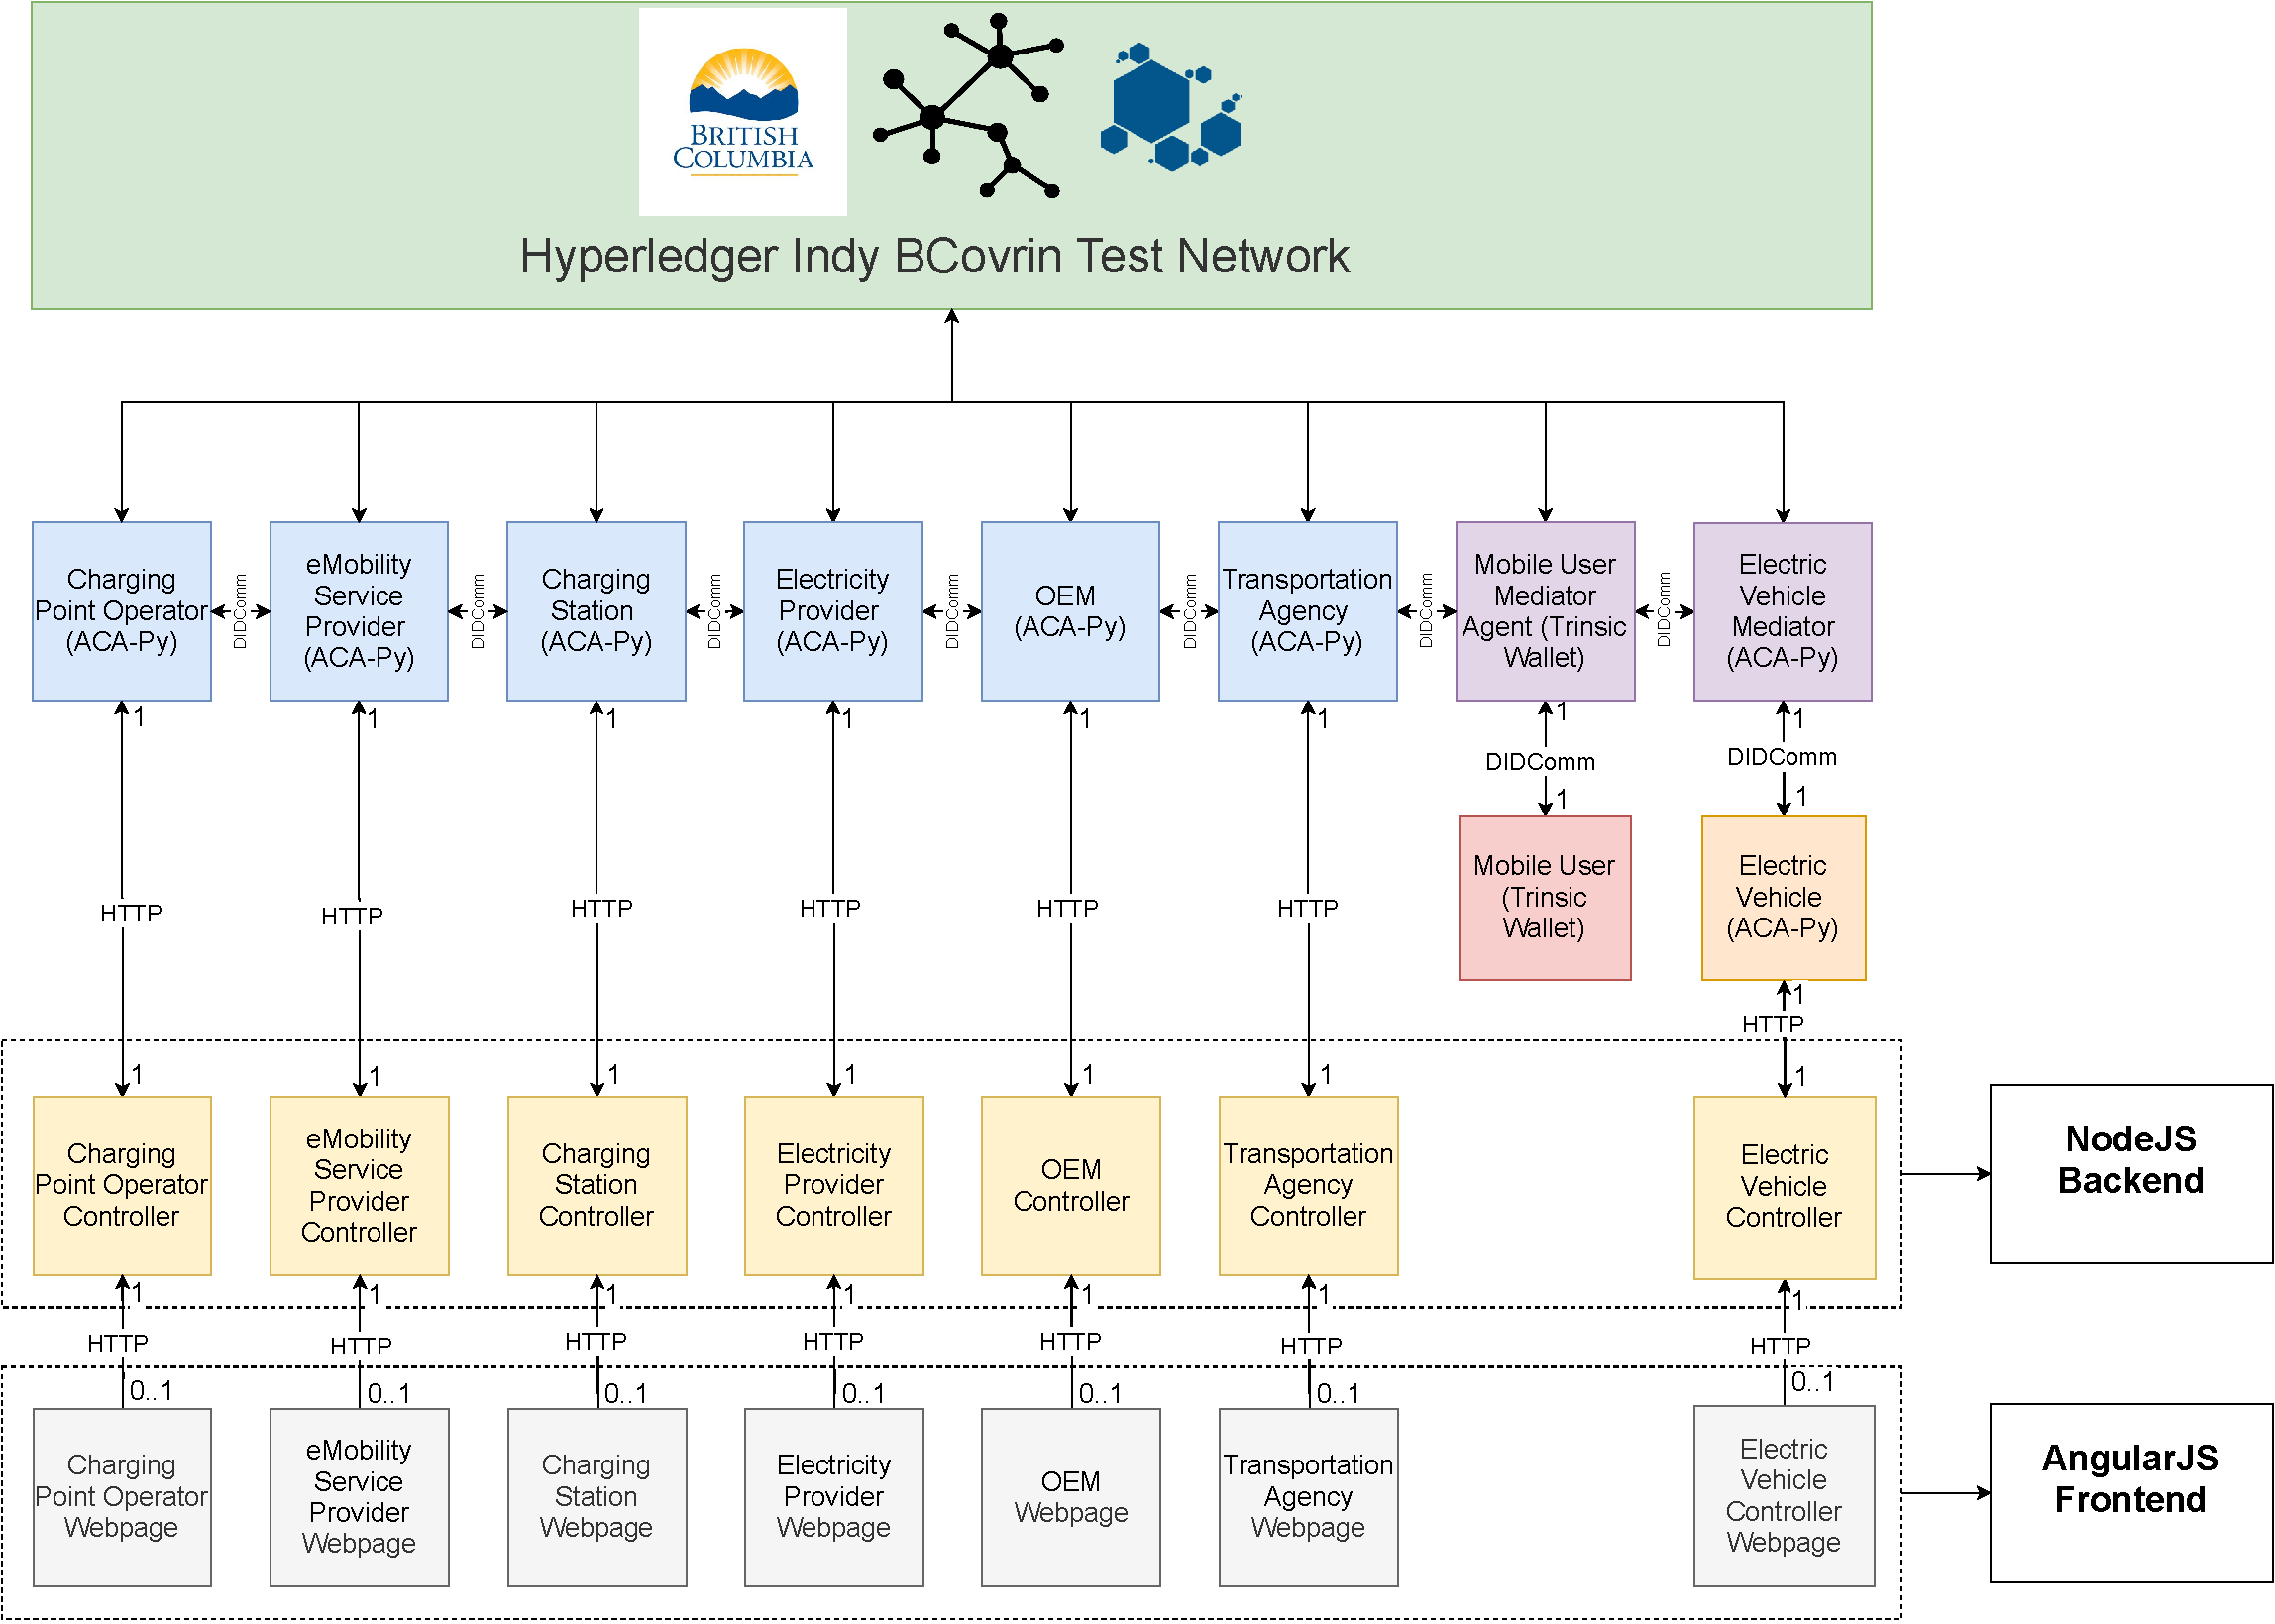
\includegraphics[keepaspectratio=true, width=\textwidth]{images/ImplementationArchitecture.pdf}
    \caption{Implementation Components Architecture and Protocols}
    \label{fig:Implementation_Architecture}
\end{figure}

\subsubsection{Agent Configuration}
\label{subsubsec:agent_configuration}

The parameters used to start-up the agents play a significant role in the necessary tasks needed to be performed by the controller (and in turn the developer). Within the content found on the ACA-Py repository, there are a great number of deployment parameters that can be set on startup. Here the configuration details of the agents are discussed and rationalized. For more information on each of the parameters it is recommended to look at the official startup parameters documentation\footnote{\url{https://github.com/hyperledger/aries-cloudagent-python/blob/main/DevReadMe.md\#about-aca-py-command-line-parameters}}. 

One of the most important things to mention in these parameters is the fact that for the sake of simplification and given that this implementation was created with the goal of being a proof-of-concept, multiple "auto-*" parameters have been set to true. This allows the agent to automatically perform certain actions, without the need of a controller. Although this helps demonstrate the functionalities of the agents, in a production level application it would be better to manually implement these actions.
% The following list of parameters was extracted from one example agent (the CPO agent), with the only parameters in need to change for the other agents being highlighted with an asterisk (*). 
In cases of mediation, if this connection is meant to be established on startup (which is the case with this proof-of-concept), then the \textit{open-mediation} and \textit{mediator-invitation} parameters needs to be set on the mediator and the mediated agents, respectively.

It is also relevant to mention that the agents have pre-configured webhook functionalities, that allow for a better interaction with the agents. After assigning a \textit{webhook-url} (which in theory should be assigned to the same endpoint as the controller that is running), it is possible to listen to specific webhook URLs and extract information about the different steps in the communications, and from that perform custom logic using the controller. One example of that is the basic messages exchanged between the CS and the CPO agents to obtain the charging rate fee (as depicted in Figure~\ref{fig:charging_and_billing_ssd} of Section~\ref{subsubsec:information-flows-ssi}).

\iffalse

\begin{itemize}
    \item General (for all agents)
    \begin{itemize}
        \item admin-insecure-mode: true
        \item admin: [0.0.0.0, 8018] *
        \item label: cpo.Agent *
        \item inbound-transport: - [http, 0.0.0.0, 8017] *
        \item outbound-transport: http
        \item endpoint: http://cpoagent10.ejemplo.me *
        \item genesis-url: http://test.bcovrin.vonx.io/genesis 
        \item seed: 0923456ERFDZSXCVTYUO9986OREDFCPO *
        \item auto-provision: true
        \item wallet-type: indy
        \item wallet-name: cpoWallet *
        \item wallet-key: 12345678 *
        \item tails-server-base-url: http://host.docker.internal:6543
        \item webhook-url: http://host.docker.internal:9229/cpo/webhooks *
        \item auto-accept-invites: true
        \item auto-accept-requests: true
        \item auto-ping-connection: true
        \item auto-respond-messages: true
        \item auto-respond-credential-proposal: true
        \item auto-respond-credential-offer: true
        \item auto-respond-credential-request: true
        \item auto-respond-presentation-proposal: true
        \item auto-respond-presentation-request: true
        \item auto-verify-presentation: true
        \item auto-store-credential: true
    \end{itemize}
    \item For Mediator Agents
    \begin{itemize}
        \item open-mediation: true
    \end{itemize}
    \item For Mediated Agents
    \begin{itemize}
        \item mediator-invitation: "http://evmediatoragent10.ejemplo.me?oob=eyJAd....fV19"
    \end{itemize}
\end{itemize}

\fi

\subsubsection{Adopted Aries RFCs}
\label{subsubsec:adopted_aries_rfcs}

All standards used in this solution follow the Aries RFCs Specifications (which have been marked as ACCEPTED at the time of writing) found in the appropriate GitHub repository\footnote{\url{https://github.com/hyperledger/aries-rfcs/blob/master/index.md}}. These RFCs are considered to be the standard for communication between Aries agents. The most relevant RFCs that explain how the agents can establish connections, send messages, issue credentials, verify credentials, be mediated, are highlighted below with a link to the appropriate RFC:

\begin{itemize}
    \item \textbf{Aries RFC 160: Connection Protocol} - In order for an agent to establish a connection with another, the communication flow follows the Aries RFC 160: Connection Protocol\footnote{\url{https://github.com/hyperledger/aries-rfcs/blob/master/features/0160-connection-protocol/README.md}}.
    \item \textbf{Aries RFC 095: Basic Message} - When an agent sends a message to another agent, it utilizes the Aries RFC 0095 - Basic Message\footnote{\url{https://github.com/hyperledger/aries-rfcs/blob/master/features/0095-basic-message/README.md}}.
    \item \textbf{Aries RFC 0036: Issue Credential Protocol 1.0} - The first iteration of the Issue Credential Protocol is used to explain the flow of messages needed to issue credentials from one agent to another. This protocol is still utilized in this proposed solution despite the introduction of version 2.0 of this RFC, since the Trinsic Wallet App only supports versions 1.0 of the protocols mentioned in this section\footnote{\url{https://github.com/hyperledger/aries-rfcs/blob/master/features/0036-issue-credential/README.md}}.
    \item \textbf{Aries RFC 0037: Present Proof Protocol 1.0} - This is the sibling RFC to the RFC 0036, since this utilizes the concepts explained in the latter to explain how a Holder can prove to a Verifier (remembering the roles explained in Section~\ref{subsubsec:verifiable_credential_model}) any claims\footnote{\url{https://github.com/hyperledger/aries-rfcs/blob/master/features/0037-present-proof/README.md}}.
    \item \textbf{Aries RFC 0453: Issue Credential Protocol 2.0} - The second iteration of the Issue Credential Protocol is used when an ACA-Py agent wishes to issue credentials to other ACA-Py agents. This version replaces the (indy-specific) filtration criteria with a generalized filter attachment to align with the rest of the messages in the protocol\footnote{\url{https://github.com/hyperledger/aries-rfcs/blob/master/features/0453-issue-credential-v2/README.md}}.
    \item \textbf{Aries RFC 0454: Present Proof Protocol 2.0} - As a second iteration of the Present Proof Protocol 1.0 protocol, this one is used between presentation requests between ACA-Py agents, since both support the usage of this protocol\footnote{\url{https://github.com/hyperledger/aries-rfcs/blob/master/features/0454-present-proof-v2/README.md}}.
    \item \textbf{Aries RFC 0046: Mediators and Relays} - In order to guarantee mediation between agents, used in the Electric Vehicle agent implementation, the communication flow between mediator and mediated agents is explained in detail in RFC 0046: Mediators and Relays\footnote{\url{https://github.com/hyperledger/aries-rfcs/blob/master/concepts/0046-mediators-and-relays/README.md}}.
    \item \textbf{Other Relevant RFCs} - Other RFCs are implicitly used when developing using the Aries framework, and are underlying to the agents communications. Therefore they have been abstracted from a detailed explanation but are worth revisiting in the official Aries RFCs repository as linked in the introduction to this section.
\end{itemize}

\subsubsection{Application Logic}
\label{subsubsec:application_logic}

Since the application relies on multiple parties, it is important to explain how the flow between the \textit{frontend - backend - agent} works, with the help of some use cases. The agents expose REST API endpoints which are used to trigger operations according to the agents documentation, as explained previously in Section~\ref{subsubsec:agent_configuration}. The controllers are all present in the same NodeJS project, which essentially has different endpoints, depending on the action that is meant to be performed, as in any REST API application. To provide a better understanding of how the application works, a small diagram in Figure~\ref{fig:flow_of_credential_issuance} contains the call stack between the different components in the use case of the Charging Station issuing a credential to the EVOwner at the end of the charging session.

\begin{figure}[!htb]
    \centering
    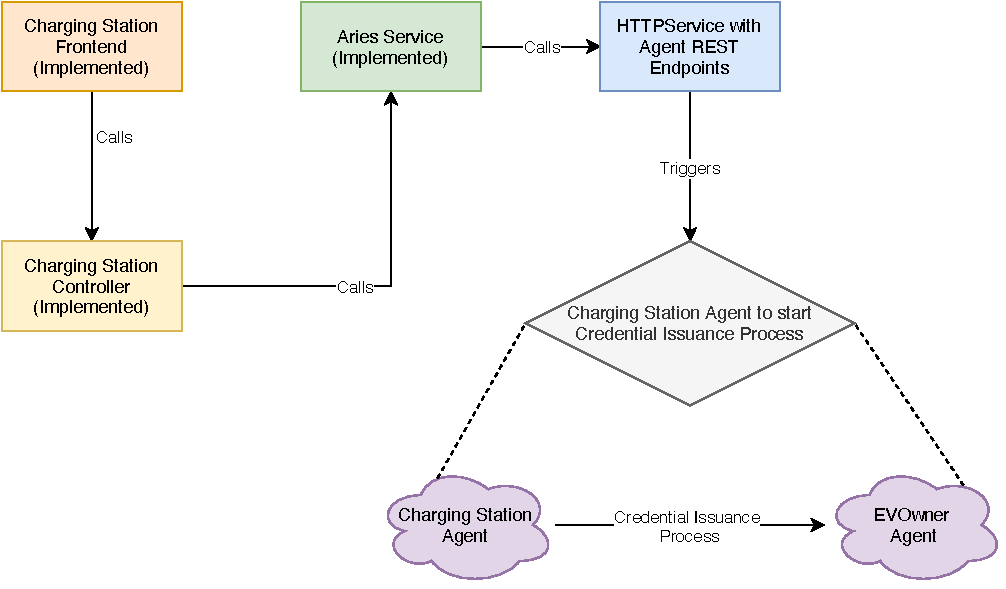
\includegraphics[keepaspectratio=true, width=0.8\textwidth]{images/FlowOfCredentialIssuance.pdf}
    \caption{Call stack to Start Credential Issuance Process}
    \label{fig:flow_of_credential_issuance}
\end{figure}

Starting off, the user triggers the action to issue the credential by pressing the button on the UI "Issue Receipt Credential". This will trigger the AngularJS function \textit{issueCredential} (as seen below) that will call the Angular Service to hit a NodeJS REST endpoint that is tailored for that event (function \textit{issueCredentialWithFields}). 

\begin{lstlisting}[language=JavaScript]
  issueCredential(): any {
    this.coreService.issueCredentialWithFields('cs', this.connectionId, 'receipt', this.eMSPContractID);
  }
\end{lstlisting}

\begin{lstlisting}[language=JavaScript]
  public issueCredentialWithFields(endpointName: string, connectionId: string, credentialEndpoint: string, contractID: string): any {
    try {
      return this.http.post(this.backendUrl + '/' + endpointName + '/issue-credential/' + credentialEndpoint, {"connectionId": connectionId, "eMSPContractID": contractID}, this.headers).toPromise();
    } catch (err) {
      console.log(err);
    }
  }
\end{lstlisting}

The code below is the controller code on the NodeJS backend that is listening to the endpoint hit previously by the frontend call (\textit{issue-credential/receipt}). Lines 4-10 represent the object that contains the attribute values for the receipt credential after a charging session. The object \textit{credentialOffer} in line 14 represents the object that is sent to the issuer agent, with information such as the connectionID (line 16) to the (to-be) holder of said credential. Other relevant information like the schemaID, credential definition ID and issuer DID (lines 21-23) are also present in this object. At last, the object is ready to be sent to the appropriate agent endpoint that handles the issuance of credentials. For this, the controller calls the implemented service (line 27) to perform the HTTP POST request that are used to interact with the agents.

\begin{lstlisting}[language=JavaScript]
    @Post('issue-credential/receipt')
    public issueCredentialReceipt(@Body("connectionId") connectionToEVOwner: any, @Body("eMSPContractID") eMSPContractID: any): Promise<CredentialExchange> {

        var credentialValues = [
            "0000000001",
            "00:30:00",
            this.currentChargingRate,
            "4€",
            eMSPContractID
        ]

        const credentialPreviewArray = this.credential7schema_attributes.map((key, i) => ({ name: key, value: credentialValues[i] }));

        const credentialOffer = new CredentialProposalRequestV1(false,
            "Charging Transaction Receipt",
            connectionToEVOwner,
            new CredentialPreview('issue-credential/1.0/credential-preview', credentialPreviewArray),
            {
                dif: { some_dif_criterion: '' },
                indy: {
                    schema_id: this.credential7schema_id,
                    cred_def_id: this.credential7credentialDefinitionID,
                    issuer_did: this.csDID
                }
            });

        return new Promise(resolve => {
            this.ariesService.sendCredentialV1(this.api, credentialOffer).pipe()
                .subscribe(responseSend => {
                    resolve(responseSend);
                }
                )
        }
        )
    }
\end{lstlisting}

After the service is called, the service is programmed to make use of the agents REST endpoints and have them perform the desired tasks, in the code below it is possible to see the generic implementation of how to have an agent start the issuance of credentials (with the V1 protocol version). After this point, the agent will handle the rest and the credential will be sent to the receiver agent.

\begin{lstlisting}[language=JavaScript]
        public sendCredentialV1(endpoint: string, credentialProposalRequest: CredentialProposalRequestV1): Observable<CredentialExchange> {
        return this.httpService
            .post(endpoint + "issue-credential/send", credentialProposalRequest)
            .pipe(map((response: AxiosResponse<CredentialExchange>): CredentialExchange => response.data))
            .pipe(
                catchError(e => {
                    throw new HttpException(e.response.data, e.response.status);
                }));
    }
\end{lstlisting}

\subsection{Deployment Details}
\label{subsec:deployment_details}

In this section the deployment details of the prototype will be highlighted, with instructions on how to replicate the behaviour of the system and what conditions to bear in mind when deploying the system from fresh. 

\subsubsection{Steps for the deployment}
\label{subsubsec:steps_for_the_deployment}

In order to deploy the system, a number of software/utilities are used. The system comprises of 6 components, which are containerized using Docker\footnote{\url{https://www.docker.com/}} and orchestrated using docker-compose\footnote{\url{https://docs.docker.com/compose/install/}}. These components are present in Figure~\ref{fig:docker-desktop} and contain the following:

\begin{itemize}
    \item postgres - a container that is running an instance of a postgres database, needed in case of backend persistent storage (if needed, to keep track of connection IDs, schema IDS and/or credential definition IDs).
    \item docker - this entry contains two instances that make for one tails-server\footnote{\url{https://github.com/bcgov/indy-tails-server}}, which is used as the revocation registry for the system, this is necessary otherwise revocation cannot be supported. This software stores and makes available tails files for use with Hyperledger Indy.
    \item aries-cloudagent-containers - this is an entry that comprises all eight agents that were created for this proof-of-concept, each agent is therefore a docker container.
    \item ssi-thesis-backend - a container that is running a NodeJS backend with the NestJS\footnote{\url{https://nestjs.com/}} framework, for the backend of the proof-of-concept.
    \item ssi-thesis-frontend - four containers that are running multiple instances of AngularJS\footnote{\url{https://angular.io/}} frontends, one for the main application, and three used to have a better interface of three of the agents states (connections, credentials, etc...).
\end{itemize}

\begin{figure}[!htb]
    \centering
    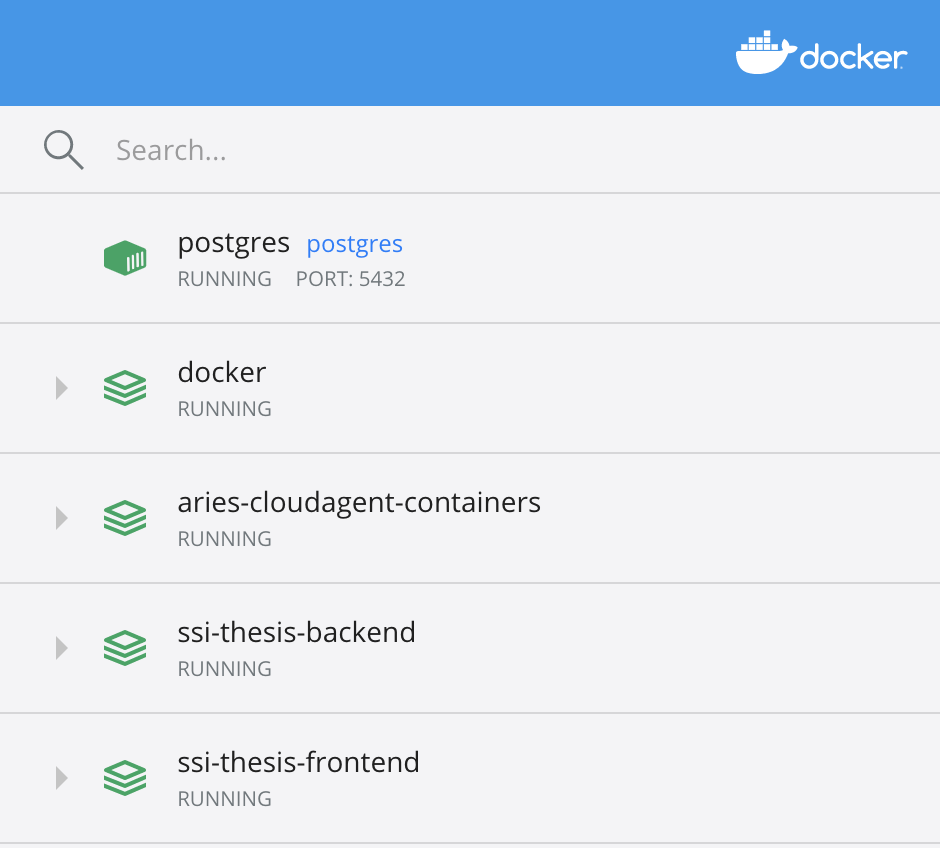
\includegraphics[keepaspectratio=true, width=0.5\linewidth]{images/docker-desktop.png}
    \caption{Docker Desktop with running containers}
    \label{fig:docker-desktop}
\end{figure}

In order to deploy these containers, the instructions are put together in different bash scripts\footnote{Used to curl specific endpoints to automate connections, issuance and verification of credentials for testing and demonstration purposes.} to automate the deployment of the application.

Given that the agents need to know how to interact with others using their own endpoints (or through the mediators endpoints), in a development environment these endpoints would be \textit{localhost:port}. But, to be able to access them from the outside, it was decided that using a tunneling software would make the solution more elegant and more close to reality. For this purpose, the open-source software pgrok\footnote{\url{https://github.com/jerson/pgrok}} was used. It offers free introspected tunnels to localhost, and this way the agents have their own fixed endpoint. 

For instructions on how to install the Trinsic Wallet Agent Mobile Application, please refer to the instructions on Appendix~\ref{app:trinsic_installation}, where a detailed description on how to setup the agent is provided.

The best source of code documentation is present in the GitHub repository that complements this manuscript. It contains all the necessary information on how to deploy the system and where changes need to be made depending on different scenarios.
Despite those instructions, a step-by-step guide will also be provided below.

\paragraph{Step 1: pgrok configuration}

To make sure the agents have their tunnels active before the start of the application, running the following line will start the tunneling service for each agent. This deployment follows the configuration created that will forward each agent's localhost port to a specific endpoint, exclusive for each agent. 

\begin{lstlisting}
pgrok -config=pgrok.yml start oemagent epagent evmediatoragent rdwagent csagent evagent emspagent cpoagent 
\end{lstlisting}

\begin{figure}[!htb]
    \centering
    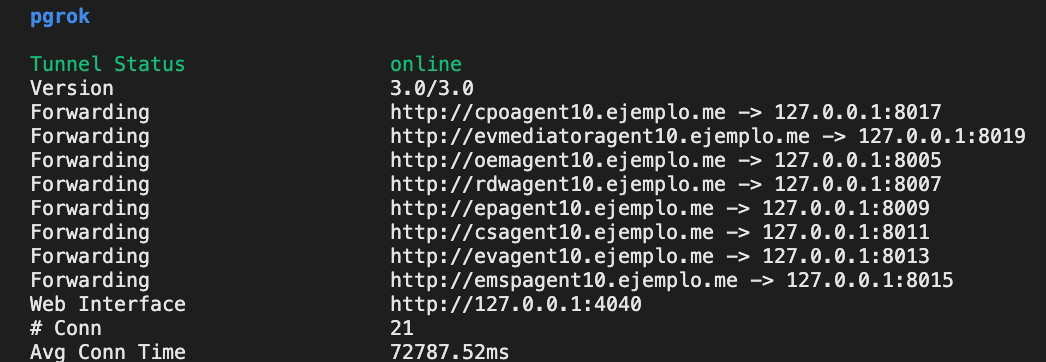
\includegraphics[width=0.6\linewidth]{images/pgrok.jpeg}
    \caption{pgrok in action, tunneling the localhost ports to specific endpoints, depending on the configuration}
    \label{fig:pgrok_image}
\end{figure}

\paragraph{Step 2: Configuration File}
This file is crucial for the systems operation. It is located in the backend implementation (\textit{ssi-thesis-backend/src/common/config/DefaultConfig.ts}). This is where the hard-coded information is written to, and from where the controller extracts information regarding:

\begin{itemize}
    \item Agents endpoints;
    \item Public DIDs;
    \item Credential Schema IDs and Credential Definition IDs;
    \item Connection IDs
\end{itemize}

\paragraph{Step 3: \textit{deployment.sh} script}

This script is in charge of deploying the revocation registry (tails-server), the agents, the backend, the postgres instance and the frontends.
Each agent is deployed according to a configuration file specific to each agent.
There is a particular step that is really important for the deployment of the agents. On startup, the mediator agent for the Electric Vehicle will create a mediation-invitation. This is printed in the command line and needs to be pasted to the \textit{mediator-invitation} field on the EVs agent deployment configuration file (\textit{ev.config.yml}). After pasting the mediatior-invitation to the configuration and pressing enter on the terminal, the deployment will carry on and both the EV and EV mediator agents mediation will be established.

\paragraph{Step 4: \textit{establish\_connections.sh} script}

For the sake of demonstrating the functionalities of the system, the agents connections are setup using a script, and the connection IDs are stored in a file for the agents to communicate between themselves. This script makes HTTP calls to the controller and that in turn makes contact with the agents to first create the connection invitations on the inviting agent, and receive the connection invitation on the receiver agent.
Each connection ID that is printed (as seen in Figure~\ref{fig:connections_screenshot}) needs to be pasted on the correct field on the Configuration File, as explained before.

\begin{figure}[!htb]
    \centering
    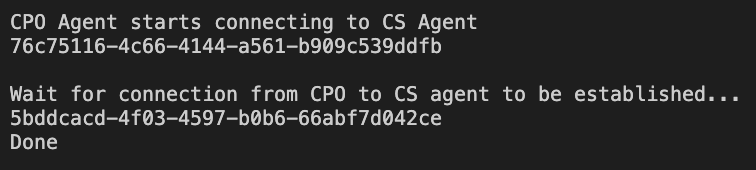
\includegraphics[width=0.6\linewidth]{images/connections_screenshot.png}
    \caption{How to extract the connection IDs after executing the script}
    \label{fig:connections_screenshot}
\end{figure}

\paragraph{Step 5: \textit{deploy\_schemas\_and\_credential\_definitions} script}

After setting the version number in the Configuration file (field "schema\_version"), the task of submitting schemas and credential definitions onto the ledger has been automated. The REST API calls the controller to create the schemas by making the calls to the agents' endpoints, this way the appropriate agent submits these onto the ledger (according to Table~\ref{tab:mapping_of_credentials} in Section~\ref{subsubsec:schemas_and_CDs}). Similar to the previous \textit{establish\_connections.sh} script, the shell script outputs the Schema IDs and the Credential Definition IDs that should be inserted into the Configuration file, as presented in Figure~\ref{fig:schemas_screenshot}.

\begin{figure}[!htb]
    \centering
    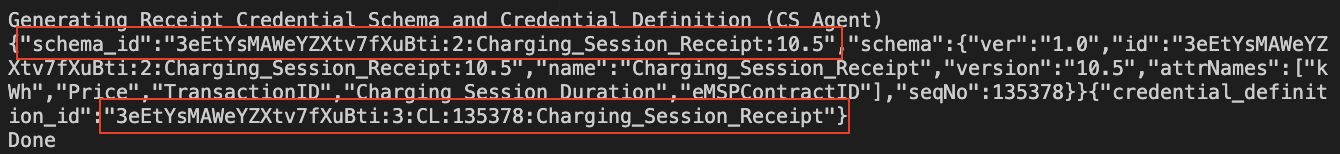
\includegraphics[width=0.8\linewidth]{images/schema_and_credential_definition.png}
    \caption{How to extract the schema and credential definition IDs after executing the script}
    \label{fig:schemas_screenshot}
\end{figure}


\subsubsection{Steps for running the use case scripts}
\label{subsubsec:steps_for_running_the_use_case_scripts}

After deploying the system, it is ready to power the use cases described in Section~\ref{subsubsec:information-flows-ssi}. The tasks that are conducted only between ACA-Py agents have been automated via shell scripts to hit the specific controller endpoints to trigger specific actions. All of the actions that require EV Owner interactions are meant to be used by means of the frontend instances deployed.

\paragraph{Step 1: \textit{service\_providers\_flow.sh} script}

This script triggers the "Service Providers Flow" explained in Section~\ref{paragraph:service_providers_flows_with_ssi}, only from the eMSP, CPO, EP and CS perspectives.

It starts with the eMSP issuing the Contract with CPO credential to the CPO.

\begin{lstlisting}[language=bash]
#Issue Contract with CPO to CPO from EMSP (CREDENTIAL 5)
curl -s -XPOST -H "Content-type: application/json" 'localhost:9229/emsp/issue-credential/cpo' > /tmp/output.html

printf '\nCredential is being issued from EMSP to CPO...\n'
sleep 2
printf '\nDone\n'
\end{lstlisting}

Then the CPO issues a credential to the Charging Station to attest its ownership.

\begin{lstlisting}[language=bash]
#Issue Ownership of CS to CS from CPO (CREDENTIAL 6)
curl -s -XPOST -H "Content-type: application/json" 'localhost:9229/cpo/issue-credential/ownership-cs' > /tmp/output.html

printf '\nCredential is being issued from CPO to CS...\n'
sleep 2
printf '\nDone\n'
\end{lstlisting}

And at last, the EP issues a Contracting Credential to the CPO.

\begin{lstlisting}[language=bash]
#Issue Contract with CPO to CPO from EP (CREDENTIAL 8)
curl -s -XPOST -H "Content-type: application/json" 'localhost:9229/ep/issue-credential/contract-cpo' > /tmp/output.html

printf '\nCredential is being issued from EP to CPO...\n'
sleep 2
printf '\nDone\n'
\end{lstlisting}

To complete the rest of the use case, the EV Owner performs the steps listed below. Note that visual representations of each step can be found in Appendix~\ref{subapp:service_providers_flow}:

\begin{enumerate}
    \item Navigate to the frontend's URL (localhost:4200)
    \item Select the eMSP portal (Figure~\ref{fig:service_provider_screenshot_1}).
    \item Connect to the TA Agent using the QR Code, scanning it with the Trinsic Wallet App (Figure~\ref{fig:service_provider_screenshot_2}).
    \item Press the "Issue Credential" button (Figure~\ref{fig:service_provider_screenshot_3}) and accept the credential on the Trinsic Wallet App (Figure~\ref{fig:service_provider_screenshot_4}).
\end{enumerate}

\paragraph{Step 2: \textit{ev\_interactions.sh} script}

This script triggers the "EV Owner and EV Interactions with SSI" explained in Section~\ref{paragraph:ev_owner_and_ev_interactions_with_ssi}, only from the EV, OEM and TA perspective.

It starts with the OEM agent issuing the VIN Credential to the Electric Vehicle.

\begin{lstlisting}[language=bash]
#Issue VIN Credential to EV from OEM (CREDENTIAL 1)
curl -s -XPOST -H "Content-type: application/json" 'localhost:9229/oem/issue-credential/send' > /tmp/output.html
printf '\nCredential is being issued from OEM to EV...\n'
sleep 2
printf '\nDone\n'
\end{lstlisting}

Then, the TA verifies this credential, and issues another credential to attest the EVs registration.

\begin{lstlisting}[language=bash]
#RDW Verify VIN Credential and Issue EV Registration to EV from RDW (CREDENTIAL 2)
printf '\nRDW is requesting VIN credential from EV\n'
curl -s -XPOST -H "Content-type: application/json" 'localhost:9229/rdw/present-proof/send-request'  > /tmp/output.html
printf '\nRequest sent, waiting for reply from EV\n'
\end{lstlisting}

To complete the rest of the use case, the EV Owner performs the steps listed below. Note that visual representations of each step can be found in Appendix~\ref{subapp:ev_owner_and_ev_interactions}:

\begin{enumerate}
    \item Navigate to the frontend's URL (localhost:4200)
    \item Select the TA portal (Figure~\ref{fig:ev_owner_screenshot_1}).
    \item Connect to the TA Agent using the QR Code, scanning it with the Trinsic Wallet App (Figure~\ref{fig:ev_owner_screenshot_2}).
    \item Press the "Issue Credential" button (Figure~\ref{fig:ev_owner_screenshot_3}) and accept the credential on the Trinsic Wallet App (Figure~\ref{fig:ev_owner_screenshot_4}).
\end{enumerate}

\paragraph{Step 3: Performing the "Charging and Billing" flow}

This part of the system does not rely on any scripts, but rather just the EV Owner interacting with the frontend and the Trinsic Wallet App.

The steps are already described in Section~\ref{paragraph:charging_and_billing_flow_with_ssi}, but a link between the steps and the screenshots of the frontend and the Trinsic Wallet App will be made below, similarly to what was done for the previous two scripts above.

To complete this use case, the EV Owner performs the steps listed below. Note that visual representations of each step can be found in Appendix~\ref{subapp:charging_and_billing}:

\begin{enumerate}
    \item Navigate to the frontend's URL (localhost:4200)
    \item Select the Charging Station Dashboard (Figure~\ref{fig:charging_screenshot_1.0}).
    \item Connect to the Charging Station Agent using the QR Code, scanning it with the Trinsic Wallet App (Figure~\ref{fig:charging_screenshot_1.1}).
    \item Press the "Request Proofs" button (Figure~\ref{fig:charging_screenshot_2}).
    \item Receive the two presentation requests (Figure~\ref{fig:charging_screenshot_3}), and accept the Request for the Contract with eMSP credential (Figure~\ref{fig:charging_screenshot_3.1}) and the EV Owner Registration at the TA one (Figure~\ref{fig:charging_screenshot_3.2}).
    \item At the Charging Station Dashboard, press the "Verify Proofs" button (Figure~\ref{fig:charging_screenshot_4}).
    \item The credentials have now been verified by the agent as seen on the screen, as well as the eMSP Company name is presented on the screen (Figure~\ref{fig:charging_screenshot_5}).
    \item Now that the Company Name is known, the EV Owner may request the current charge rate pressing the "Obtain Current Charge Rate" button (Figure~\ref{fig:charging_screenshot_6}).
    \item The price/kWh is presented on the screen (Figure~\ref{fig:charging_screenshot_7}).
    \item The EV Owner presses "Request EV Credentials" (Figure~\ref{fig:charging_screenshot_8}) so that the Charging Station can request from the EV agent a presentation to attest it is the same vehicle as indicated by the EV Owner.
    \item After a few seconds, the EV Owner presses "Verify Proofs" to verify if the process has been concluded.
    \item The credential from the EV has now been verified by the CS agent as seen on the screen, as well as the registration number is presented on the screen together with the EV Owner registration number (Figure~\ref{fig:charging_screenshot_9}).
    \item Now the EV Owner may start charging the EV, pressing the "Start Charging" button (Figure~\ref{fig:charging_screenshot_10}).
    \item The Charging Station will start the charging and stop it right away (Figure~\ref{fig:charging_screenshot_11}).
    \item The EV Owner can now issue a receipt credential, pressing the "Issue Receipt Credential" button (Figure~\ref{fig:charging_screenshot_12}).
    \item On the Trinsic Wallet App, the EV Owner will receive a credential offer (Figure~\ref{fig:charging_screenshot_13}).
    \item The EV Owner accepts the credential by clicking the "Accept" button (Figure~\ref{fig:charging_screenshot_14.0}) and the credential is stored on the Trinsic Wallet App (Figure~\ref{fig:charging_screenshot_14.1}).
    \item An overview of the final state of the Charging Station dashboard in the good-case scenario can be found in Figure~\ref{fig:charging_screenshot_15}.
\end{enumerate}



